\documentclass[10pt]{beamer}

\usepackage[francais]{babel}
\usepackage[utf8x]{inputenc}
\usepackage[T1]{fontenc}
\usepackage{bookman}
\usepackage{amsmath}
\usepackage{amscd}
\usepackage{amssymb}
\usepackage{amsthm}
\usepackage{latexsym}
\usepackage{graphicx}
\usepackage{color}
\usepackage{xcolor}
\usepackage{calc}
\usepackage{setspace}
\usepackage[boxruled,vlined,french]{algorithm2e}
\usepackage{times}
\usepackage{tikz}
\usepackage{verbatim}

%\setlength{\voffset}{-3.75cm}
%\setlength{\hoffset}{-2.6cm}
%\setlength{\oddsidemargin}{2.75cm}
%\setlength{\topmargin}{2in}
%\setlength{\headheight}{0in}
%\setlength{\headsep}{0in}
%\setlength{\topskip}{0in}
\setlength{\parindent}{0cm}
%\setlength{\parskip}{1ex plus0.4ex minus0.2ex}
%\setlength{\textwidth}{16.25cm}
%\setlength{\textheight}{21cm}
%\renewcommand{\baselinestretch}{1.5}
\flushbottom
\setcounter{page}{1}
\setcounter{tocdepth}{1}

\SetKw{Edb}{Effet de bord}
\SetKw{Et}{et}
\SetKw{Ou}{ou}
\SetKw{De}{de}
\SetKw{A}{à}
\SetKwBlock{Debut}{Début}{Fin}
\SetKwIF{Si}{SinonSi}{Sinon}{Si}{alors}{Sinon si}{Sinon}{FinSi}
\SetKwFor{Pour}{Pour}{faire}{FinPour}
\SetKwFor{PourTout}{Pour tout}{faire}{FinPour}
\SetKwFor{TantQue}{Tant que}{faire}{FinTantQue}
\SetKw{Retour}{retourner}


\newcommand{\guill}[1]{«~#1~»}

\usetikzlibrary{arrows,shapes}



\usetheme{Singapore}

\AtBeginSection[]
{
  \begin{frame}<beamer>
    \frametitle{Plan}
    \tableofcontents[currentsection]
  \end{frame}
}

\defbeamertemplate*{footline}{infolines theme}
{
 \hbox{
  \begin{beamercolorbox}[wd=.22\paperwidth,ht=2.25ex,dp=1ex,center]{author in head/foot}%
    \insertshortauthor%
  \end{beamercolorbox}%
  \begin{beamercolorbox}[wd=.57\paperwidth,ht=2.25ex,dp=1ex,center]{title in head/foot}%
    \insertshorttitle%
  \end{beamercolorbox}%
  \begin{beamercolorbox}[wd=.13\paperwidth,ht=2.25ex,dp=1ex,center]{date in head/foot}%
    \insertshortdate{}%
  \end{beamercolorbox}%
  \begin{beamercolorbox}[wd=.08\paperwidth,ht=2.25ex,dp=1ex,center]{author in head/foot}%
    \insertframenumber/\inserttotalframenumber%
  \end{beamercolorbox}}%
}



\title[Analyse de suites d'accords de jazz]{\large \\ Rapport de stage \Large Analyse de suites d'accords de jazz}
\institute{ENS de Lyon, M1 Informatique fondamentale}

\author[R. Versaevel]{\normalsize Romain \textsc{Versaevel}\newline \\ \normalsize Encadré par Pr. David \textsc{Meredith}}

\date{\today}

\begin{document}


\begin{frame}
\titlepage
\end{frame}

\begin{frame}{Plan}
\tableofcontents
\end{frame}

\section{LZ77}

\begin{frame}{LZ77: exemple}
\begin{block}{Entrée}
$\texttt{I}=ABCABCABD$
\end{block}

\bigskip

\only<2> {
\begin{tabular}{|c|c|c|c|c|c|c|c|c|c|c|c|c|c|c|c|c|c|c|}
\hline
\textbf{Étape}&\multicolumn{9}{|c|}{\textbf{Buffer}} & \multicolumn{9}{|c|}{\textbf{Entrée} (\guill{Aperçu})} \\
\hline
0&&&&&&&&&&A&B&C&A&B&C&A&B&D\\
\hline
\end{tabular}}

\only<3> {
\begin{tabular}{|c|c|c|c|c|c|c|c|c|c|c|c|c|c|c|c|c|c|c|}
\hline
\textbf{Étape}&\multicolumn{9}{|c|}{\textbf{Buffer}} & \multicolumn{9}{|c|}{\textbf{Entrée} (\guill{Aperçu})} \\
\hline
0&&&&&&&&&&A&B&C&A&B&C&A&B&D\\
\hline
1&&&&&&&&&A&B&C&A&B&C&A&B&D&\\
\hline
\end{tabular}}

\only<4> {
\begin{tabular}{|c|c|c|c|c|c|c|c|c|c|c|c|c|c|c|c|c|c|c|}
\hline
\textbf{Étape}&\multicolumn{9}{|c|}{\textbf{Buffer}} & \multicolumn{9}{|c|}{\textbf{Entrée} (\guill{Aperçu})} \\
\hline
0&&&&&&&&&&A&B&C&A&B&C&A&B&D\\
\hline
1&&&&&&&&&A&B&C&A&B&C&A&B&D&\\
\hline
2&&&&&&&&A&B&C&A&B&C&A&B&D&&\\
\hline
\end{tabular}}

\only<5> {
\begin{tabular}{|c|c|c|c|c|c|c|c|c|c|c|c|c|c|c|c|c|c|c|}
\hline
\textbf{Étape}&\multicolumn{9}{|c|}{\textbf{Buffer}} & \multicolumn{9}{|c|}{\textbf{Entrée} (\guill{Aperçu})} \\
\hline
0&&&&&&&&&&A&B&C&A&B&C&A&B&D\\
\hline
1&&&&&&&&&A&B&C&A&B&C&A&B&D&\\
\hline
2&&&&&&&&A&B&C&A&B&C&A&B&D&&\\
\hline
3&&&&&&&A&B&C&A&B&C&A&B&D&&&\\
\hline
\end{tabular}}

\bigskip

\begin{block}{Sortie}
$\textbf<2>{(0,0,A)}$,
$\textbf<3>{(0,0,B)}$,
$\textbf<4>{(0,0,C)}$,
$\textbf<5>{(3,5,D)}$
\end{block}
\end{frame}

\begin{frame}{LZ77 : décompression}
\begin{block}{Entrée}
$\texttt{I}=ABCABCABD$
\end{block} \bigskip

\begin{tabular}{ll}
Décompression & Compression \\
\uncover<3->{$A$} & $\textbf<2,3>{(0,0,A)}$ \\
\uncover<5->{$B$} & $\textbf<4,5>{(0,0,B)}$ \\
\uncover<7->{$C$} & $\textbf<6,7>{(0,0,C)}$ \\
\uncover<9->{$A$} & $\textbf<8,9,10,11>{(3,5,D)}$ \\
\uncover<9->{$B$} & \\
\uncover<9->{$C$} & \\
\uncover<10->{$A$} & \\
\uncover<10->{$B$} & \\
\uncover<11->{$D$} & \\
\end{tabular}
\end{frame}


\subsection{Diagonal patterns}

\begin{frame}{Diagonal patterns (1)}
\begin{figure}
\centering
\only<1>{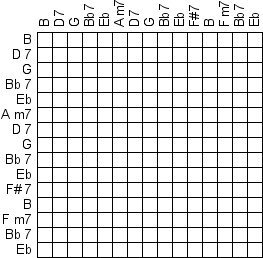
\includegraphics[width = 6cm]{images/diagonals0.jpg}}
\only<2>{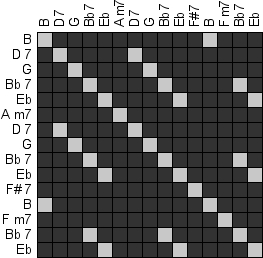
\includegraphics[width = 6cm]{images/diagonals1.jpg}}
\only<3>{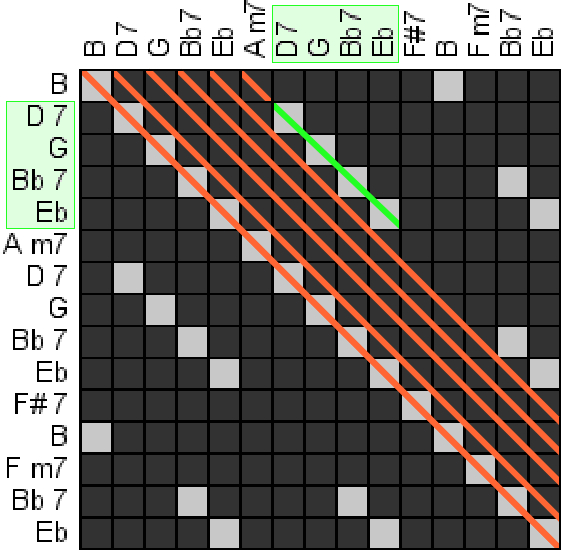
\includegraphics[width = 6cm]{images/diagonals2.jpg}}
\end{figure}
\end{frame}


\begin{frame}{Diagonal patterns (2)}
\begin{itemize}
\item[Step 1] Identify the patterns
\item[Step 2] Find a (small) cover
\end{itemize}
\end{frame}

\begin{frame}{Diagonal patterns (3)}
\begin{block}{Input}
$\texttt{I}=
B;D 7;G;B\flat 7;E\flat;A m7;D 7;G;B\flat 7;E\flat;F\# 7;B;F m7;B\flat 7;E\flat$
\end{block} \pause

\begin{block}{Patterns}
\begin{itemize}
\item[$\triangleright$] $B$ --- $\{0;11\}$;
\item[$\triangleright$] $B\flat 7;~E\flat$ --- $\{3;8;13\}$;
\item[$\triangleright$] $D7;~G;~B\flat 7;~E\flat$ --- $\{1;6\}$; \pause
\item[$\triangleright$] $D7$ --- $\{1;6\}$, $G$ --- $\{2;7\}$\dots
\end{itemize}
\end{block} \pause

\begin{block}{Output}
\begin{itemize}
\item[$\triangleright$] $B$ --- $\{0;11\}$;
\item[$\triangleright$] $B\flat 7;~E\flat$ --- $\{13\}$;
\item[$\triangleright$] $D7;~G;~B\flat 7;~E\flat$ --- $\{1;6\}$;
\item[$\triangleright$] $Am7$ --- $\{5\}$, $F\#7$ --- $\{10\}$, $Fm7$ --- $\{12\}$
\end{itemize}
\end{block}
\end{frame}

\begin{frame}{Diagonal patterns (4)}
\begin{figure}
\centering
\only<1>{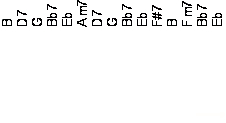
\includegraphics[width = 8cm]{images/cover0.jpg}}
\only<2>{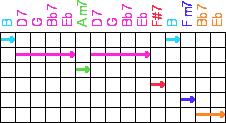
\includegraphics[width = 8cm]{images/cover1.jpg}}
\end{figure}
\end{frame}

\section{Mesures de similarité}
\subsection{Similarity measures}

\begin{frame}{The magical ingredient}
\begin{align*}
\Large
C & = C' \\
\uncover<2> {
& \downarrow \\
C &\sim C'}
\end{align*}
\end{frame}


\begin{frame}{All measures}
\begin{itemize}
\item[$\triangleright$] root note equivalence;
\item[$\triangleright$] transposition equivalence;
\item[$\triangleright$] PCS-Prime equivalence;
\item[$\triangleright$] the F1-score;
\item[$\triangleright$] Isaacson's similarity index;
\item[$\triangleright$] Lewin's measure;
\item[$\triangleright$] Morris' measure;
\item[$\triangleright$] Rahn's measure;
\item[$\triangleright$] Teitelbaum's measure.
\end{itemize}
\end{frame}

\begin{frame}{Thresholds}
\begin{figure}
\centering

\includegraphics[width = 8cm]{images/threshold.jpg}
\end{figure}
\end{frame}




\section{Résultats}

\begin{frame}{Evaluation}
\begin{block}{Compression factor}
\Large \uncover<2>{
$\frac{|\text{Input}|}{|\text{Output}|}$}
\end{block}

\bigskip

\begin{block}{Recovery factor}
\Large \uncover<2>{
$\frac{|\{i~|~\textsc{decompress}(\textsc{compress}(\text{Input}))[i] = \text{Input}[i]\}|}{|\text{Input}|}$ }
\end{block}
\end{frame}


\subsection{Comparison between measures}

\begin{frame}{Comparison between measures (1)}
\begin{block}{ }
\Large
« Similarity measures are similar. » \pause
\end{block}

\begin{figure}
\centering
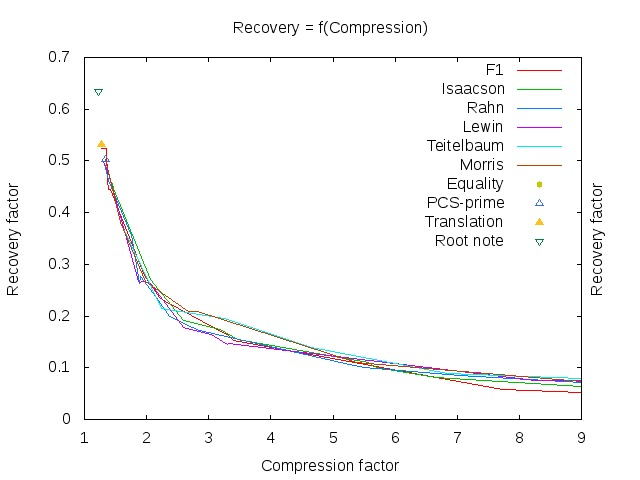
\includegraphics[width = 7cm]{images/RfC77.jpg}
\end{figure}
\end{frame}


\begin{frame}{Comparison between measures (2)}
\only<1> {
\begin{figure}
\centering
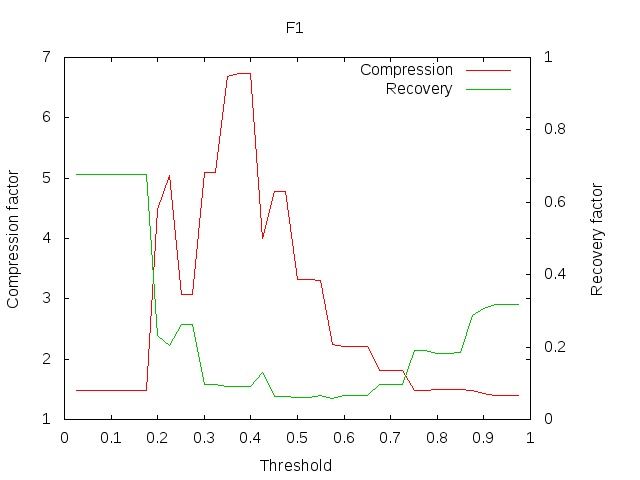
\includegraphics[width = 5cm]{images/F1Diag.jpg} \hspace{0.5cm}
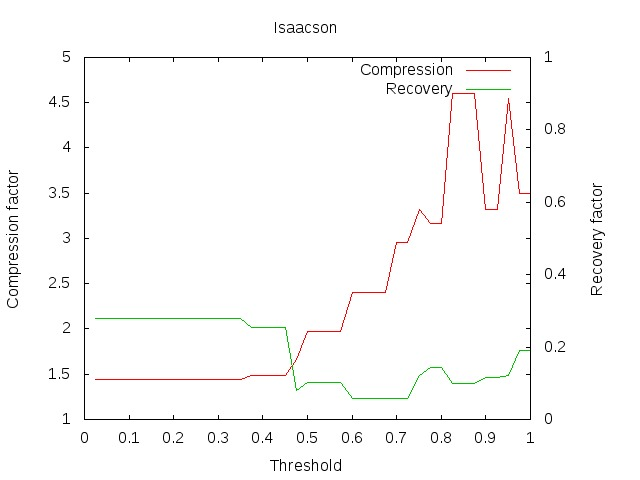
\includegraphics[width = 5cm]{images/IsaacsonDiag.jpg}
\end{figure}}

\only<2> {
\begin{figure}
\centering
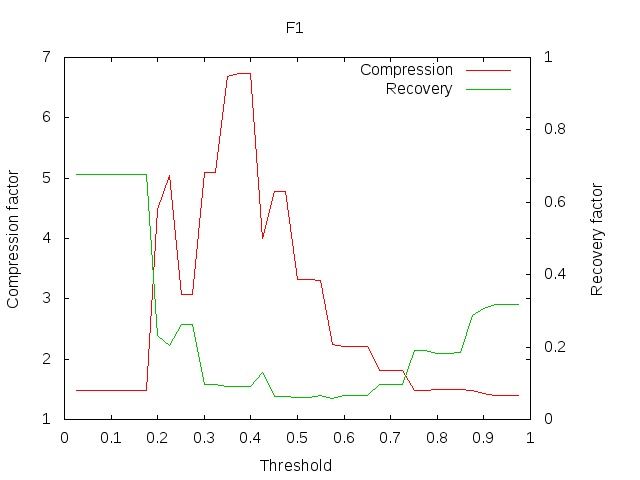
\includegraphics[width = 9cm]{images/F1Diag.jpg}
\end{figure}}

\only<3> {
\begin{figure}
\centering
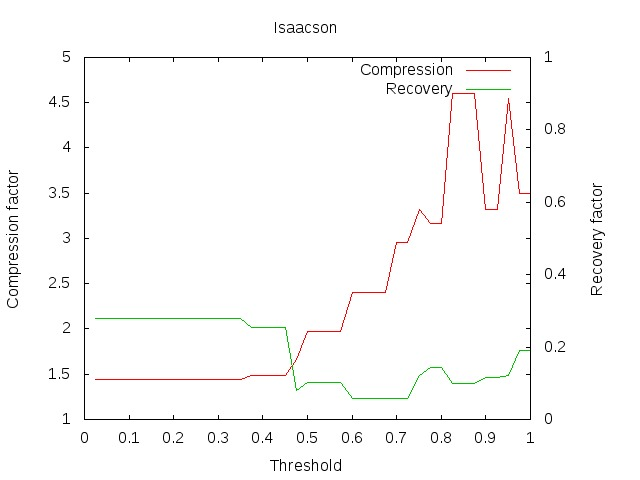
\includegraphics[width = 9cm]{images/IsaacsonDiag.jpg}
\end{figure}}
\end{frame}



\subsection{Comparison between algorithms}


\begin{frame}{Comparison between algorithms (1)}
\only<1> {
\begin{figure}
\centering
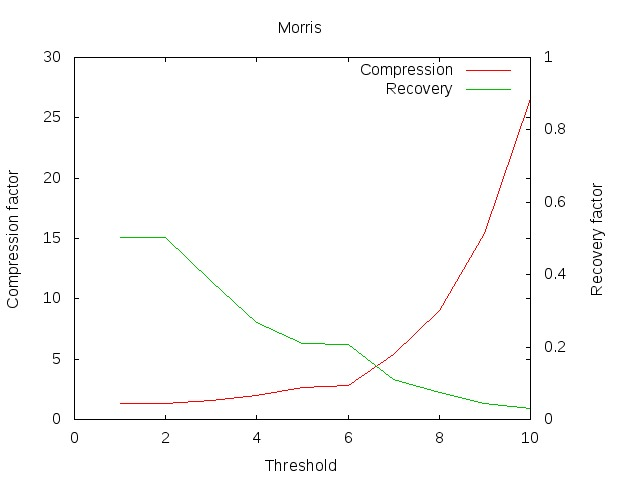
\includegraphics[width = 5cm]{images/Morris77.jpg} \hspace{0.5cm}
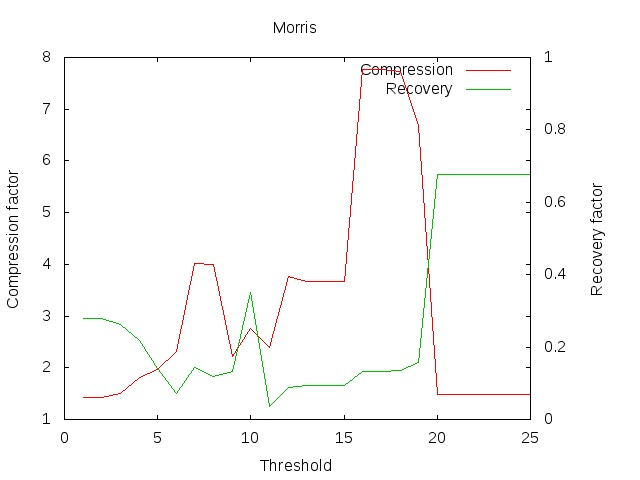
\includegraphics[width = 5cm]{images/MorrisDiag.jpg}
\end{figure}}

\only<2> {
\begin{figure}
\centering
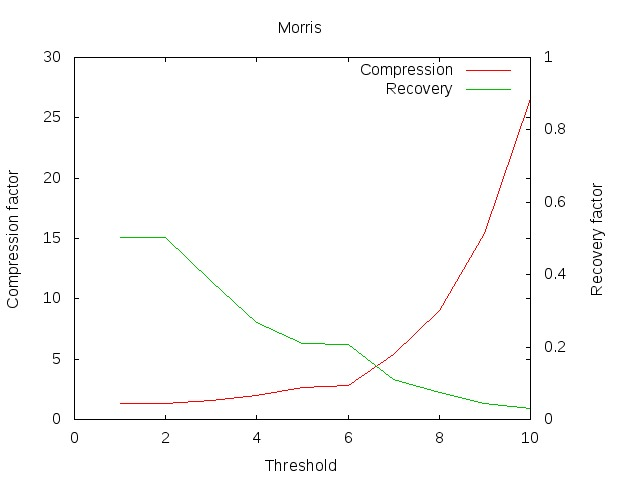
\includegraphics[width = 9cm]{images/Morris77.jpg}
\end{figure}}

\only<3> {
\begin{figure}
\centering
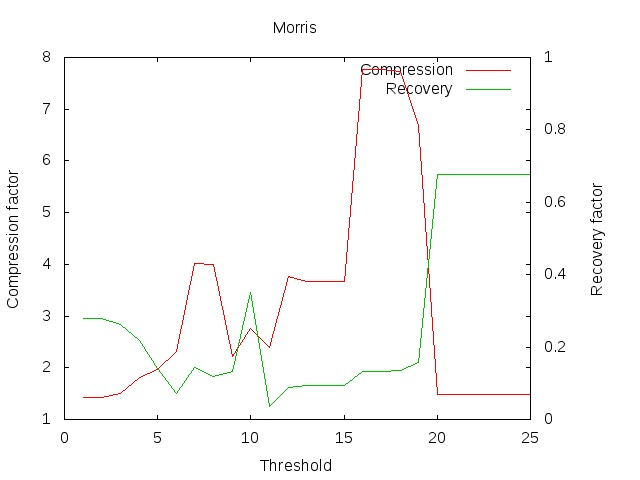
\includegraphics[width = 9cm]{images/MorrisDiag.jpg}
\end{figure}}
\end{frame}



\begin{frame}{Comparison between algorithms (2)}
\only<1> {
\begin{figure}
\centering
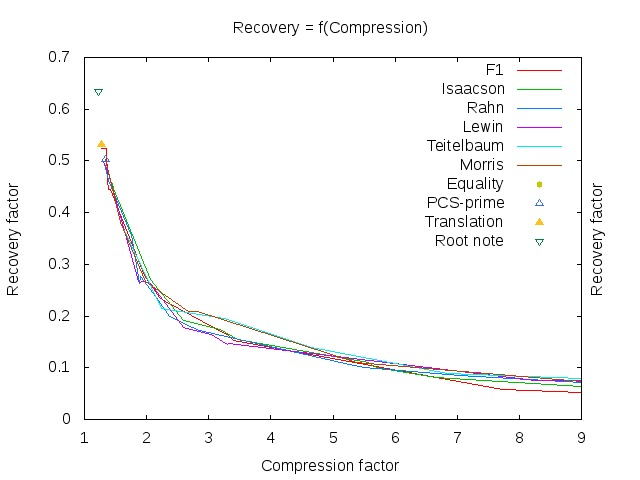
\includegraphics[width = 5cm]{images/RfC77.jpg} \hspace{0.5cm}
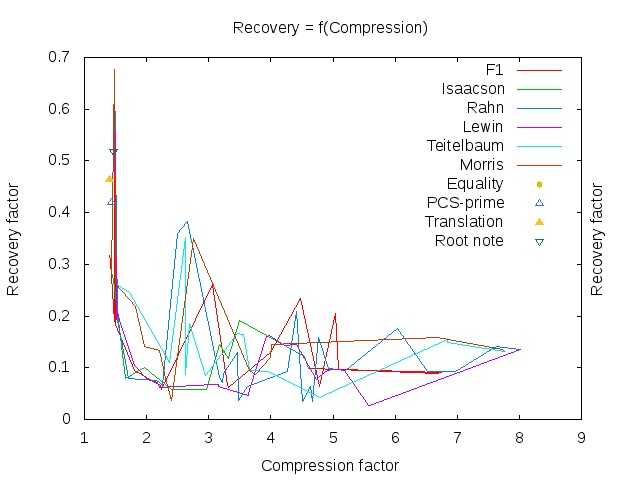
\includegraphics[width = 5cm]{images/RfCDiag.jpg}
\end{figure}}

\only<2> {
\begin{figure}
\centering
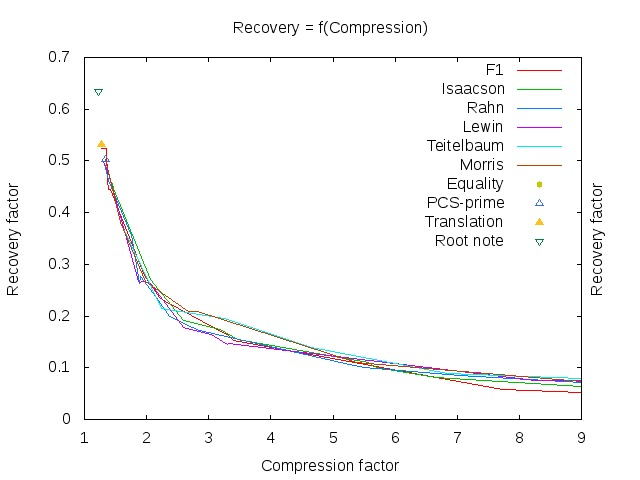
\includegraphics[width = 9cm]{images/RfC77.jpg}
\end{figure}}

\only<3> {
\begin{figure}
\centering
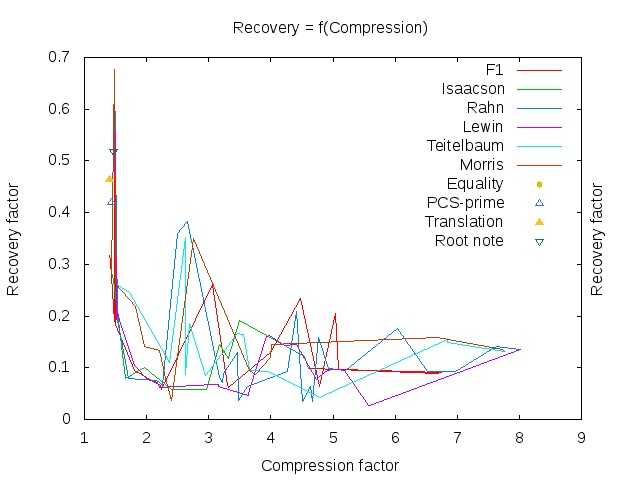
\includegraphics[width = 9cm]{images/RfCDiag.jpg}
\end{figure}}
\end{frame}



\begin{frame}
\begin{figure}
\centering

\includegraphics[width = 10cm]{images/taf.jpg}
\end{figure}
\end{frame}

\end{document}













